\begin{frame}{La tentation de la désintermédiation}
    \begin{itemize}
        \item Précarisation des écrivain.es 
        \item Tensions avec les grands éditeur.rices 
        \item Mise à disposition d'outils d'auto-publication/édition 
    \end{itemize}
    \textrightarrow{} place de l'éditeur.rice au sein de l'écosystème éditorial?\\
    \vspace{1em}
    \textbf{Concept de la désintermédiation}\\
    Gallezot Gabriel et Ertzscheid Olivier, \textit{« Swaper la publication »}, 2006: "[...] pour l'autopublication, il faut ajouter "sans intermédiaire"" dans le processus de publication.
\end{frame}

\begin{frame}{Qu'entend-t-on par désintermédiation?}
    \begin{enumerate}
        \item Un concept économique dès les années 60 avec le développement de techniques numériques.
        \item Établissement d'une relation directe entre une entité (industrielle, culturelle, institutionnelle) et ses usagers entraînant la disparition de certains services.
    \end{enumerate}
    \textrightarrow{} Renvoie à \textbf{la disparition de certains intermédiaires} qui incarnaient une forme d'autorité, ou qui conféraient cette autorité\\
    = les édteur.rices, les grands distributeurs, les libraires etc...
\end{frame}
\begin{frame}{Exemple: les critiques littéraires}
    \begin{figure}
        \centering
        
\includegraphics[width=.4\textwidth]{images/masque_plume.png}
        \hspace{1em}
        
\includegraphics[width=.4\textwidth]{images/babelio.png}
    \end{figure}
\end{frame}
\begin{frame}{Exemple: les critiques littéraires}
    \begin{block}{Booktube, BookTok, Bookstagram}
        \begin{figure}
            \centering
            
\includegraphics[width=.45\textwidth, height=5cm]{images/Bookstagram.png}
            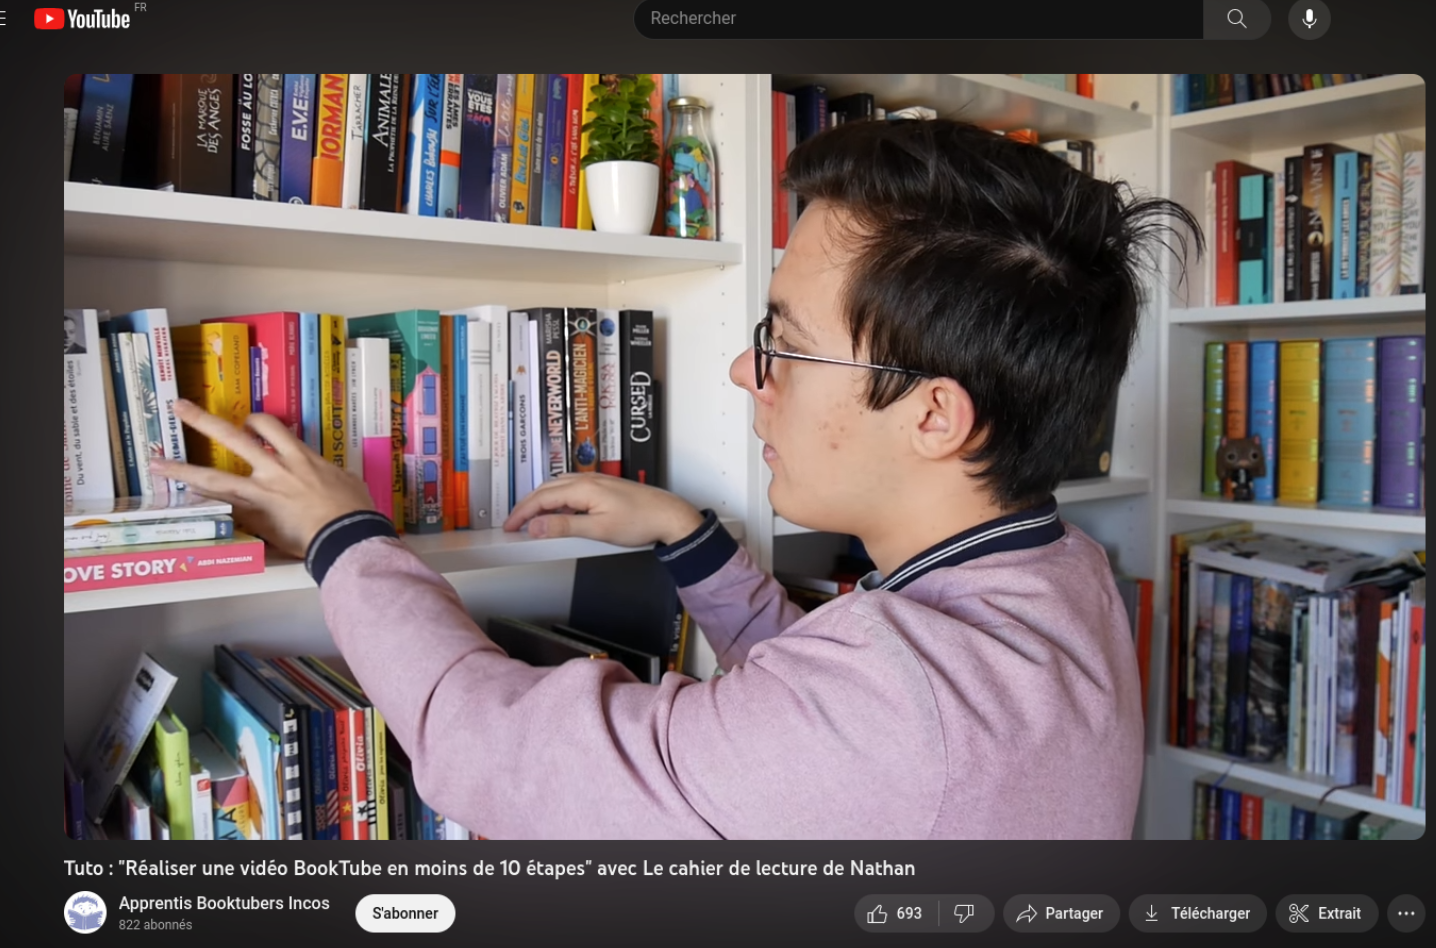
\includegraphics[width=.45\textwidth, height=5cm]{images/BookTube.png}
        \end{figure}
    \end{block}
    
\end{frame}

\begin{frame}{Exemple: les critiques littéraires}
    \begin{figure}
        \begin{center}
            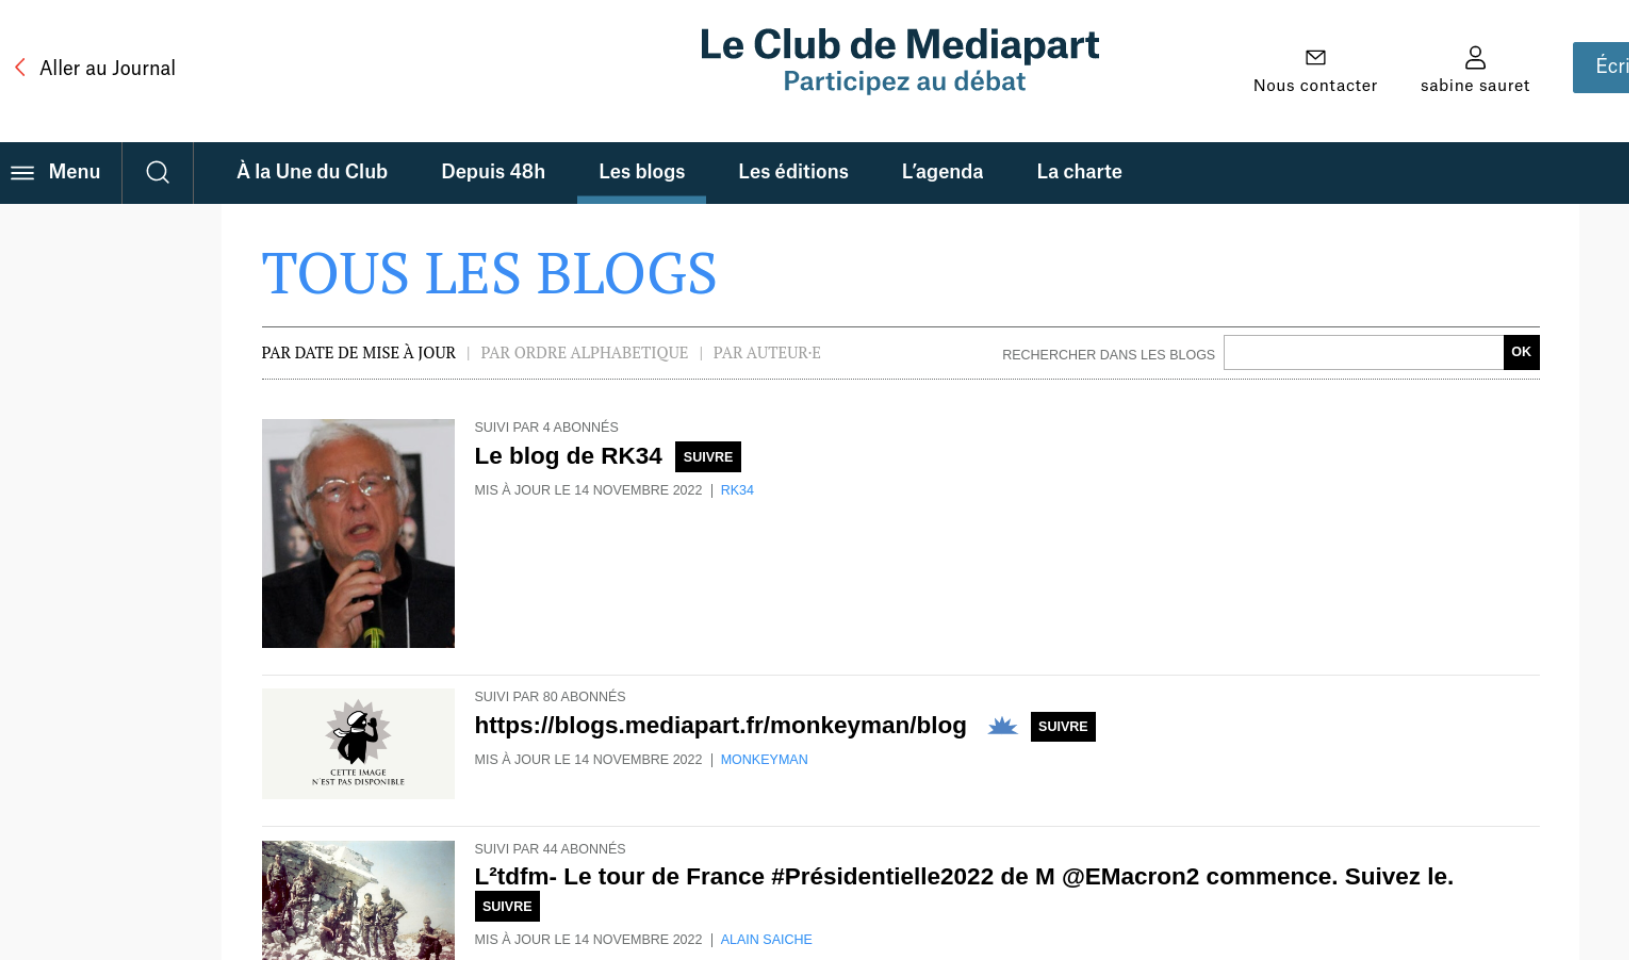
\includegraphics[width=.8\textwidth]{images/mediapart.png}
        \end{center}
    \end{figure}
\end{frame}
\begin{frame}{Remise en question des autorités ayant un fort pouvoir de légitimation}
    Désintermédiation pose de nombreuses questions en termes de système hiérarchique de valeur attribués aux contenus.
\end{frame}